\documentclass[10pt, hyperref={unicode}, compress]{beamer}
\usepackage[T1]{fontenc}
\usepackage[slovak]{babel}
\usepackage[utf8]{inputenc}
\usepackage{times} % font
\usepackage{qrcode}
\usepackage{graphics} % images
\usepackage{listings} % including python code 
\usepackage[linesnumbered, ruled, noline, czech, longend]{algorithm2e}
\usepackage{subcaption} % 2 images sidy by side
\captionsetup[subfigure]{labelformat=empty} % hide letter numbergins from subfigures

\usetheme{Dresden}
\usecolortheme{beaver}
\setbeamertemplate{footline}[frame number]
\setbeamertemplate{navigation symbols}{}  % remove slides navigation

% hiding subsection bar from https://tex.stackexchange.com/a/220149
\defbeamertemplate*{headline}{miniframes theme no subsection}
{%
  \begin{beamercolorbox}[colsep=1.5pt]{upper separation line head}
  \end{beamercolorbox}
  \begin{beamercolorbox}{section in head/foot}
    \vskip2pt\insertnavigation{\paperwidth}\vskip2pt
  \end{beamercolorbox}%
  \begin{beamercolorbox}[colsep=1.5pt]{lower separation line head}
  \end{beamercolorbox}
}
\setbeamertemplate{footline}[miniframes theme no subsection]
%%%%

% custom colors
\usecolortheme{beaver}
\definecolor{fitBlue}{RGB}{0,169,224}
\definecolor{fitGray}{RGB}{243,247,246}
\definecolor{fitDarkBlue}{RGB}{22,118,208}

\setbeamercolor*{palette tertiary}{bg=fitBlue}
\setbeamercolor{title}{fg=fitDarkBlue}
\setbeamercolor{frametitle}{fg=fitDarkBlue}
\setbeamercolor{item}{fg=fitBlue}


% external link icon by "omisson" https://tex.stackexchange.com/a/294990
\usepackage{tikz}
\newcommand{\ExternalLink}{%
    \tikz[x=1.2ex, y=1.2ex, baseline=-0.05ex]{% 
        \begin{scope}[x=1ex, y=1ex]
            \clip (-0.1,-0.1) 
                --++ (-0, 1.2) 
                --++ (0.6, 0) 
                --++ (0, -0.6) 
                --++ (0.6, 0) 
                --++ (0, -1);
            \path[draw, 
                line width = 0.5, 
                rounded corners=0.5] 
                (0,0) rectangle (1,1);
        \end{scope}
        \path[draw, line width = 0.5] (0.5, 0.5) 
            -- (1, 1);
        \path[draw, line width = 0.5] (0.6, 1) 
            -- (1, 1) -- (1, 0.6);
        }
    }


\title{Pancake sort}
\author{
    \texorpdfstring{%
        Samuel Dobroň\newline
        \url{xdobro23@stud.fit.vutbr.cz}%
        }{Samuel Dobroň}
}
\institute{
	Vysoké učení technické v~Brně \\
	Fakulta informačních technologií
}
\date{\today}

\begin{document}
    \begin{frame}
        \titlepage
    \end{frame}

    \begin{frame}{Obsah}
        \setbeamertemplate{section in toc}[circle]
        \tableofcontents[hideallsubsections]
    \end{frame}
    
    \section{Úvod}
        \begin{frame}{Motivácia}
            \textit{Ako zoradiť palacinky podľa veľkosti len pomocou špachtle.}
            \bigskip
            \begin{itemize}
                \item Radenie poľa len pomocou otáčania poľa po nejaký index,
                \item Iný prístup k~problému radenia ako majú bežné algoritmy.
            \end{itemize}
        \end{frame}

    \section{Princíp}
        \subsection{Vlastnosti}
            \begin{frame}{Vlastnosti}
                \begin{itemize}
                    \item povolená operácia je len tzv. \texttt{reverse} poľa,
                    \item cieľom je čo najmenej otočení,
                    \item pracuje in-place,
                    \item je \textbf{ne}stabilný.
                \end{itemize}
            \end{frame}
        \subsection{Algoritmus}
            \begin{frame}{Pancake sort: Algoritmus}
                \begin{itemize}
                    \item Majme pole \texttt{arr}, nech jeho dĺžka je \texttt{n},
                    \item Zníž \texttt{n} o~1, nech \texttt{c} sa rovná \texttt{n}; ak platí $c > 1$:
                    \begin{enumerate}
                        \item Nájdi index \texttt{i} najväčšieho elementu v~\texttt{arr[c]},
                        \item Otoč pole \texttt{arr} do indexu \texttt{i},
                        \item Otoč pole \texttt{arr} do indexu \texttt{c - 1},
                        \item Zníž \texttt{c} o~1, skoč na bod 1.
                    \end{enumerate}
                \end{itemize}
            \end{frame}

    \section{Ukážka}
        \subsection{Ukážka}
            \begin{frame}{Vizualizácia}
            \centering
                \begin{tikzpicture}
                    \action<1>{
                        \node (rect) at (0, 0) [draw, minimum width=0.5cm, minimum height=3cm] {4};
                        \node (rect) at (0.5, 0) [draw, minimum width=0.5cm, minimum height=1cm] {1};
                        \node (rect) at (1, 0) [draw, minimum width=0.5cm, minimum height=2.3cm] {3};
                        \node (rect) at (1.5, 0) [draw, minimum width=0.5cm, minimum height=1.5cm] {2};
                        \node (rect) at (2, 0) [draw, minimum width=0.5cm, minimum height=3.5cm] {5};
                    }
                    \action<2>{
                        \node (rect) at (0, 0) [draw, minimum width=0.5cm, minimum height=3cm] {4};
                        \node (rect) at (0.5, 0) [draw, minimum width=0.5cm, minimum height=1cm] {1};
                        \node (rect) at (1, 0) [draw, minimum width=0.5cm, minimum height=2.3cm] {3};
                        \node (rect) at (1.5, 0) [draw, minimum width=0.5cm, minimum height=1.5cm] {2};
                        \node (rect) at (2, 0) [draw, minimum width=0.5cm, minimum height=3.5cm, color=red] {5};
                    }
                    \action<3>{
                        \node (rect) at (0, 0) [draw, minimum width=0.5cm, minimum height=3cm] {4};
                        \node (rect) at (0.5, 0) [draw, minimum width=0.5cm, minimum height=1cm] {1};
                        \node (rect) at (1, 0) [draw, minimum width=0.5cm, minimum height=2.3cm] {3};
                        \node (rect) at (1.5, 0) [draw, minimum width=0.5cm, minimum height=1.5cm] {2};
                        \node (rect) at (2, 0) [draw, minimum width=0.5cm, minimum height=3.5cm, color=red] {5};
                        \draw
                            (-0.25, -2) -- (1.75, -2);
                        \draw
                            (-0.25, -2.2) -- (-0.25, -1.8);
                        \draw
                            (1.75, -2.2) -- (1.75, -1.8);
                        \node at (0.8, -2.4){\LARGE $\circlearrowright$};
                    }
                    \action<4>{
                        \node (rect) at (0, 0) [draw, minimum width=0.5cm, minimum height=1cm] {1};
                        \node (rect) at (0.5, 0) [draw, minimum width=0.5cm, minimum height=2.3cm] {3};
                        \node (rect) at (1, 0) [draw, minimum width=0.5cm, minimum height=1.5cm] {2};
                        \node (rect) at (1.5, 0) [draw, minimum width=0.5cm, minimum height=3cm] {4};
                        \node (rect) at (2, 0) [draw, minimum width=0.5cm, minimum height=3.5cm, color=red] {5};
                    }
                    \action<5>{
                        \node (rect) at (0, 0) [draw, minimum width=0.5cm, minimum height=1cm] {1};
                        \node (rect) at (0.5, 0) [draw, minimum width=0.5cm, minimum height=2.3cm] {3};
                        \node (rect) at (1, 0) [draw, minimum width=0.5cm, minimum height=1.5cm] {2};
                        \node (rect) at (1.5, 0) [draw, minimum width=0.5cm, minimum height=3cm, color=red] {4};
                        \node (rect) at (2, 0) [draw, minimum width=0.5cm, minimum height=3.5cm, color=red] {5};
                    }
                    \action<6>{
                        \node (rect) at (0, 0) [draw, minimum width=0.5cm, minimum height=1cm] {1};
                        \node (rect) at (0.5, 0) [draw, minimum width=0.5cm, minimum height=2.3cm] {3};
                        \node (rect) at (1, 0) [draw, minimum width=0.5cm, minimum height=1.5cm] {2};
                        \node (rect) at (1.5, 0) [draw, minimum width=0.5cm, minimum height=3cm, color=red] {4};
                        \node (rect) at (2, 0) [draw, minimum width=0.5cm, minimum height=3.5cm, color=red] {5};
                        \draw
                            (-0.25, -2) -- (0.75, -2);
                        \draw
                            (-0.25, -2.2) -- (-0.25, -1.8);
                        \draw
                            (0.75, -2.2) -- (0.75, -1.8);
                        \node at (0.25, -2.4){\LARGE $\circlearrowright$};
                    }
                    \action<7>{
                        \node (rect) at (0.5, 0) [draw, minimum width=0.5cm, minimum height=1cm] {1};
                        \node (rect) at (0, 0) [draw, minimum width=0.5cm, minimum height=2.3cm] {3};
                        \node (rect) at (1, 0) [draw, minimum width=0.5cm, minimum height=1.5cm] {2};
                        \node (rect) at (1.5, 0) [draw, minimum width=0.5cm, minimum height=3cm, color=red] {4};
                        \node (rect) at (2, 0) [draw, minimum width=0.5cm, minimum height=3.5cm, color=red] {5};
                    }
                    \action<8>{
                        \node (rect) at (0.5, 0) [draw, minimum width=0.5cm, minimum height=1cm] {1};
                        \node (rect) at (0, 0) [draw, minimum width=0.5cm, minimum height=2.3cm] {3};
                        \node (rect) at (1, 0) [draw, minimum width=0.5cm, minimum height=1.5cm] {2};
                        \node (rect) at (1.5, 0) [draw, minimum width=0.5cm, minimum height=3cm, color=red] {4};
                        \node (rect) at (2, 0) [draw, minimum width=0.5cm, minimum height=3.5cm, color=red] {5};
                        \draw
                            (-0.25, -2) -- (1.25, -2);
                        \draw
                            (-0.25, -2.2) -- (-0.25, -1.8);
                        \draw
                            (1.25, -2.2) -- (1.25, -1.8);
                        \node at (0.55, -2.4){\LARGE $\circlearrowright$};
                    }
                    \action<9>{
                        \node (rect) at (0.5, 0) [draw, minimum width=0.5cm, minimum height=1cm] {1};
                        \node (rect) at (1, 0) [draw, minimum width=0.5cm, minimum height=2.3cm] {3};
                        \node (rect) at (0, 0) [draw, minimum width=0.5cm, minimum height=1.5cm] {2};
                        \node (rect) at (1.5, 0) [draw, minimum width=0.5cm, minimum height=3cm, color=red] {4};
                        \node (rect) at (2, 0) [draw, minimum width=0.5cm, minimum height=3.5cm, color=red] {5};
                    }
                    \action<10>{
                        \node (rect) at (0.5, 0) [draw, minimum width=0.5cm, minimum height=1cm] {1};
                        \node (rect) at (1, 0) [draw, minimum width=0.5cm, minimum height=2.3cm, color=red] {3};
                        \node (rect) at (0, 0) [draw, minimum width=0.5cm, minimum height=1.5cm] {2};
                        \node (rect) at (1.5, 0) [draw, minimum width=0.5cm, minimum height=3cm, color=red] {4};
                        \node (rect) at (2, 0) [draw, minimum width=0.5cm, minimum height=3.5cm, color=red] {5};
                    }
                    \action<11>{
                        \node (rect) at (0.5, 0) [draw, minimum width=0.5cm, minimum height=1cm] {1};
                        \node (rect) at (1, 0) [draw, minimum width=0.5cm, minimum height=2.3cm, color=red] {3};
                        \node (rect) at (0, 0) [draw, minimum width=0.5cm, minimum height=1.5cm] {2};
                        \node (rect) at (1.5, 0) [draw, minimum width=0.5cm, minimum height=3cm, color=red] {4};
                        \node (rect) at (2, 0) [draw, minimum width=0.5cm, minimum height=3.5cm, color=red] {5};
                        \draw
                            (-0.25, -2) -- (0.75, -2);
                        \draw
                            (-0.25, -2.2) -- (-0.25, -1.8);
                        \draw
                            (0.75, -2.2) -- (0.75, -1.8);
                        \node at (0.25, -2.4){\LARGE $\circlearrowright$};
                    }
                    \action<12>{
                        \node (rect) at (0, 0) [draw, minimum width=0.5cm, minimum height=1cm] {1};
                        \node (rect) at (1, 0) [draw, minimum width=0.5cm, minimum height=2.3cm, color=red] {3};
                        \node (rect) at (0.5, 0) [draw, minimum width=0.5cm, minimum height=1.5cm] {2};
                        \node (rect) at (1.5, 0) [draw, minimum width=0.5cm, minimum height=3cm, color=red] {4};
                        \node (rect) at (2, 0) [draw, minimum width=0.5cm, minimum height=3.5cm, color=red] {5};
                    }
                    \action<13>{
                        \node (rect) at (0, 0) [draw, minimum width=0.5cm, minimum height=1cm] {1};
                        \node (rect) at (1, 0) [draw, minimum width=0.5cm, minimum height=2.3cm, color=red] {3};
                        \node (rect) at (0.5, 0) [draw, minimum width=0.5cm, minimum height=1.5cm, color=red] {2};
                        \node (rect) at (1.5, 0) [draw, minimum width=0.5cm, minimum height=3cm, color=red] {4};
                        \node (rect) at (2, 0) [draw, minimum width=0.5cm, minimum height=3.5cm, color=red] {5};
                    }
                    \action<14>{
                        \node (rect) at (0, 0) [draw, minimum width=0.5cm, minimum height=1cm, color=red] {1};
                        \node (rect) at (1, 0) [draw, minimum width=0.5cm, minimum height=2.3cm, color=red] {3};
                        \node (rect) at (0.5, 0) [draw, minimum width=0.5cm, minimum height=1.5cm, color=red] {2};
                        \node (rect) at (1.5, 0) [draw, minimum width=0.5cm, minimum height=3cm, color=red] {4};
                        \node (rect) at (2, 0) [draw, minimum width=0.5cm, minimum height=3.5cm, color=red] {5};
                    }
                \end{tikzpicture}
            \end{frame}
        
        \subsection{Video vizualizácia}
            \begin{frame}{Video vizualizácia}
                \newcommand{\VisualisationUrl}{https://www.youtube.com/watch?v=kk-\_DDgoXfk}
                \begin{figure}[!tbp]
                    \begin{subfigure}[b]{0.6\textwidth}
                    \href{\VisualisationUrl}{%
                            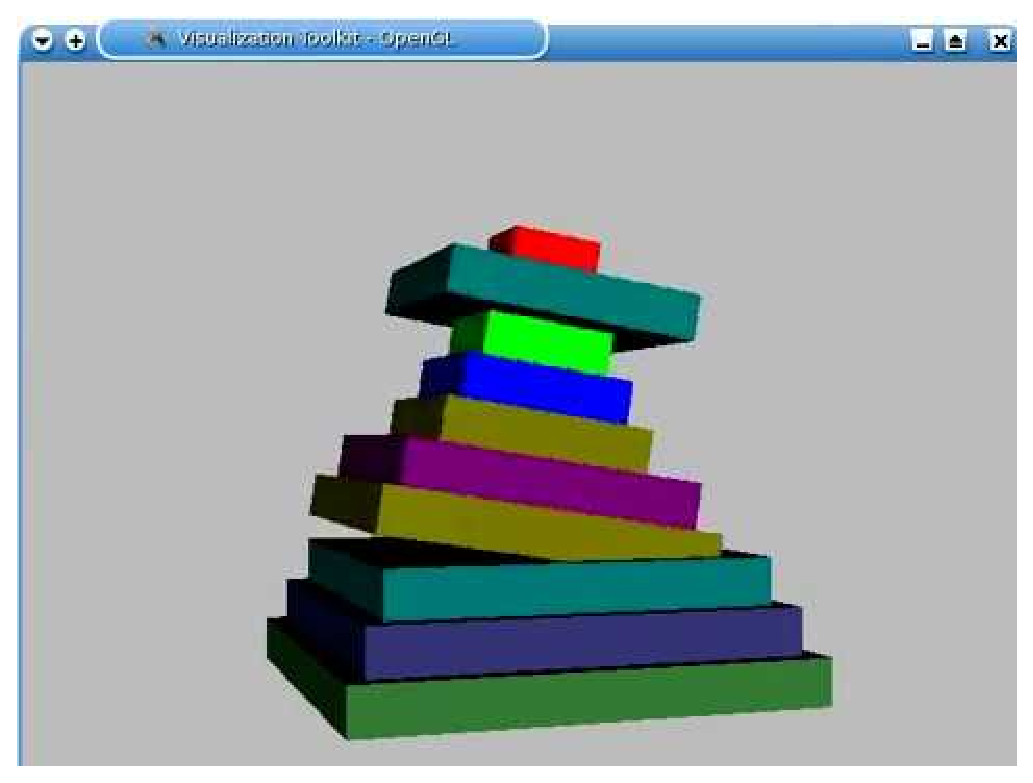
\includegraphics[width=\textwidth]{img/video.eps}%
                        }
                    \caption{Video vizualizácia}
                  \end{subfigure}%
                  %
                  \hfill%
                  %
                  \begin{subfigure}[b]{0.25\textwidth}
                    \qrcode[height=\textwidth]{\VisualisationUrl}
                    \caption{
                        \raisebox{0.5in}{\ExternalLink Youtube}
                    }
                  \end{subfigure}
                \end{figure}
            \end{frame}
    
    \section{Implementácia}
        \subsection{Pseudokód}
            \begin{frame}{Pseudokód}
                \begin{algorithm}[H]
                    \setcounter{algocf}{1}
                    \SetNlSty{textnormal}{}{:}
                    \KwIn{$(arr, arr\_len)$}
                    \KwOut{$ arr $}
                    \BlankLine
                    $n \gets c$ \\
                    \While{$c > 1$}
                    {
                        $index\_of\_max \gets findIndexOfMax(arr, c) $
                        \BlankLine
                        \If{$index\_of\_max \neq (c-1) $}{
                            reverse elemenens of $arr$ until index $index\_of\_max$ \\
                            reverse elemenens of $arr$ until index $c - 1$
                        }
                        $c \gets (c - 1)$
                    }
                    \KwRet{$arr$}
                \caption{\textsc{Pancake sort}}
                \label{algo}
                \end{algorithm}
            \end{frame}
        
        \subsection{Časová zložitosť}
            \begin{frame}{Zložitosť}
                Časová zložitosť:
                \begin{itemize}
                    \item najlepší prípad -- $\Omega(n)$
                        \begin{itemize}
                            \item už zoradené pole,
                        \end{itemize}
                    \item najhorší prípad -- $\mathcal{O}(n^2)$
                        \begin{itemize}
                            \item alternujúci najväčší a najmenší prvok -- $[0, 9, 1, 8, 2, 7, 3, 6, 5, 4]$,
                            \item treba $2n-3$ otočení.
                        \end{itemize}
                \end{itemize}
                \medskip
                Priestorová zložitosť $\mathcal{O}(n^2)$.
            \end{frame}
    
    \begin{frame}{Použité zdroje}
        \begin{itemize}
            \item Avantika Balaji: \textit{Pancake Sort Algorithm} \url{https://iq.opengenus.org/pancake-sort/}
            \item TutorialCup: \textit{Pancake Sorting Problem} \\
                \url{https://shorturl.at/kmtzW}
            \item GeeksForGeeks: \textit{Pancake sorting} \url{https://www.geeksforgeeks.org/pancake-sorting/}
        \end{itemize}
    \end{frame}

\end{document}
